 \section{Motivating Example}
\label{sec:case_study} 

%\subsubsection{Wheel Brake System}
%In order to demonstrate the fault modeling capabilities of the Safety Annex in Section~\ref{sec:fault_modeling} and provide examples of how to use the Safety Annex to perform fault modelling and analysis, we describe a model of a Wheel Brake System (WBS) of an aircraft. 

The Wheel Brake System (WBS) described in AIR6110~\cite{AIR6110} is a well-known example that has been used as a case study for safety analysis, formal verification, and contract based design~\cite{DBLP:conf/cav/BozzanoCPJKPRT15, 10.1007/978-3-319-11936-6-7, CAV2015:BoCiGrMa, Joshi05:SafeComp}. The preliminary work for the safety annex used a simplified model of the WBS~\cite{Stewart17:IMBSA}. In order to demonstrate a complex fault modeling process, we constructed a functionally and structurally equivalent AADL version of one of the most complex WBS NuSMV/xSAP models (arch4wbs) described in~\cite{DBLP:conf/cav/BozzanoCPJKPRT15}.    

\begin{figure}[h!]
	\centering
	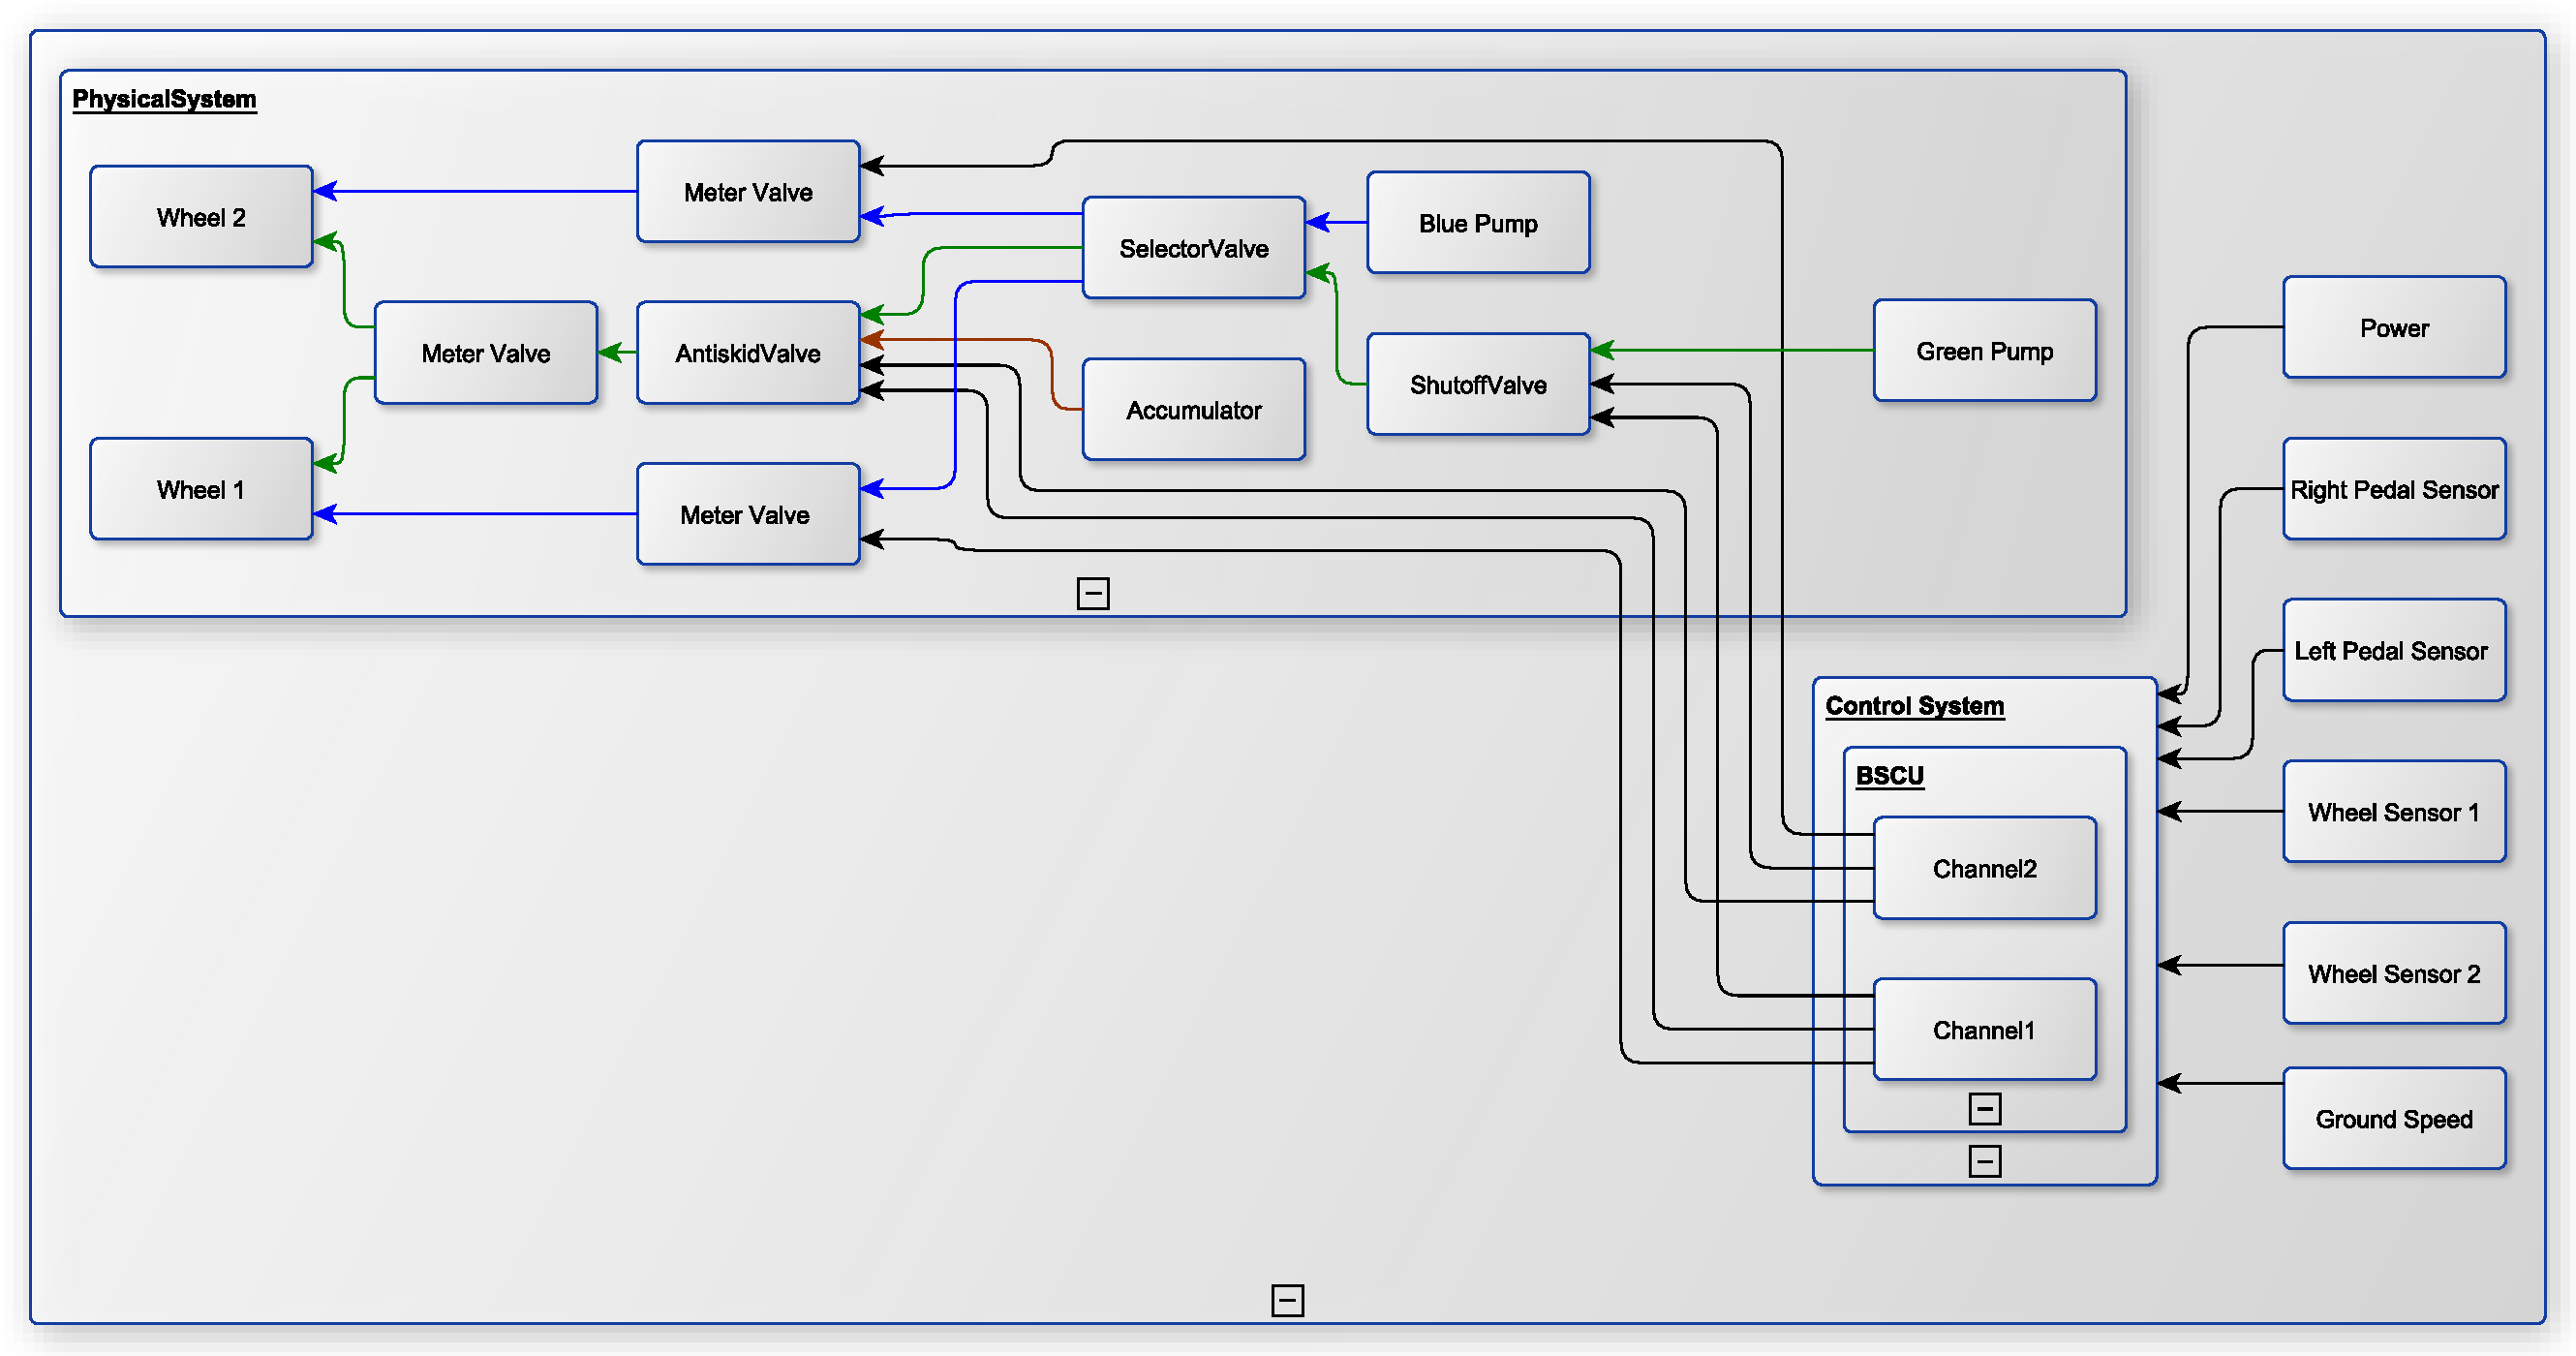
\includegraphics[trim=0 9 0 5,clip,width=\textwidth]{images/wbs_arch.pdf}
	\caption{Wheel Brake System}
	\label{fig:wbs}
\end{figure} 

%\subsubsection{WBS Architecture Description}
The WBS is composed of two main parts: the control system and the physical system. The control system electronically controls the physical system and contains a redundant channel of the Braking System Control Unit (BSCU) in case of failure. It also commands antiskid braking in case of skidding on the ground. The physical system consists of the hydraulic circuits running from hydraulic pumps to wheel brakes as well as valves that control the hydraulic fluid flow. This is what provides braking force to each of the 8 wheels of the aircraft. The wheels are all mechanically braked in pairs (one pair per landing gear). For simplicity's sake, Figure~\ref{fig:wbs} displays only two of the 8 wheels. 

There are three operating modes in the WBS model. In \textit{normal} mode, the system uses the \textit{green} hydraulic circuit. The normal system is composed of the green hydraulic pump and one meter valve per each of the 8 wheels. Each of the meter valves are controlled through electronic commands coming from the active channel of the BSCU. These signals provide braking and antiskid commands for each wheel. The braking command is determined through a sensor on the pilot pedal position and is labeled as \textit{Left/Right Pedal Sensor} in Figure~\ref{fig:wbs} and the antiskid command is determined by the \textit{Wheel Sensors}. 

In \textit{alternate} mode, the system uses the \textit{blue} hydraulic circuit. The alternate system is composed of the blue hydraulic pump, four meter valves, and four antiskid shutoff valves: one for each landing gear. The meter valves are mechanically commanded through the pilot pedal corresponding to each landing gear. If the system detects lack of pressure in the green circuit, the BSCU channel commands the selector valve to switch to the blue circuit. %This switch can occur, for example, if there is a lack of pressure from the green hydraulic pump, the green hydraulic pump circuit fails, or pressure is cut off by a shutoff valve. 
If the BSCU channel becomes invalid, the shutoff valve closes and we move into alternate mode. Once this system switches into alternate mode, it does not return to normal operation mode.

The last mode of operation of the WBS is the \textit{emergency} mode. This mode is entered if the blue hydraulic pump fails. The accumulator pump has a reserve of pressurized hydraulic fluid and will supply this to the blue circuit in emergency mode.

To get an idea of the size of this model, the system model contains 30 different kinds of components, 169 component instances, and a model depth of 5 hierarchical levels. 

The behavioral model is encoded using the AGREE annex and the behavior is based on descriptions found in AIR6110. The top level system properties are given by the requirements and safety objectives given in AIR6110. All of the subcomponent contracts support these system safety objectives through the use of assumptions on component input and guarantees on the output.

\begin{comment}
\subsubsection{WBS Behavioral Model Description}
\label{subsubsec:wbs_behavior}
The behavioral model is encoded using the AGREE annex and the behavior is based on descriptions found in AIR6110. The top level system properties are given by the requirements and safety objectives given in AIR6110. All of the subcomponent contracts support these system safety objectives by constraining subcomponent output behavior. 

Based on descriptions provided in AIR6110, the Functional Hazard Assessment (FHA) revealed a number of top level properties for the system. We will focus on one in the following sections in order to illustrate the use of the Safety Annex in fault modeling and how the behavioral propagation of faults can affect the top level safety properties of a system. 

One of the failure conditions described in AIR6110 is \textit{Inadvertent wheel braking of all wheels during takeoff roll after V1 shall be less than 1E-9 per takeoff}. Due to the catastrophic classification of this hazard, this is a property we chose for illustrative purposes. 

This property can be broken down as follows. In order for no inadvertent braking to occur, there needs to be a series of things that occur in the system simultaneously. The system is provided with both power and hydraulic pressure and the pilot has not commanded braking (by pressing the pedal). At the same time, the ground is moving (the plane is not stopped), there is braking force at the wheel, and the wheel is rolling. When all of these things happen together, this is inadvertant braking. Naturally, the safety property states this as all of these things do \textit{not} occur together. Given a model of this size, it can be complicated to determine the combinations of component errors that could occur in order to lead to a functional failure. 

In the following section, we outline the fault modelling process using the Safety Annex and illustrate using the WBS and some specific subcomponents.

%In the behavioral model, the lower level guarantees of the components serve to support the top level property. For example, in this property we have the following lower level component contracts that ensure that these behaviors of the system cannot occur simultaneously. \danielle{I need to run the lustre code using all IVCs to gather these supporting contracts. TODO: Get supporting contracts for this lemma, run analysis and see which of these supporting contracts are violated in the presence of which faults, explain the results.}


\end{comment}









